
\section{Efectuarea lucrarii de laborator}



\subsection{Tasks and Points}



 Basic Level (nota 5 $||$ 6) : 

-Realizeaza un simplu GUI calculator care suporta functiile de baza: +, -, /, *.


Normal Level (nota 7 $||$ 8):
 
-Realizeaza un simplu GUI calculator care suporta urmatoare functii: +, -, /, *, putere, radical, InversareSemn(+/-).


Advanced Level (nota 9 $||$ 10):

-Realizeaza un simplu GUI calculator care suporta urmatoare functii: +, -, /, *, putere, radical, InversareSemn(+/-), operatii cu numere zecimale.

-Divizare proiectului in doua module - Interfata grafica(Modul GUI) si Modulul de baza(Core Module).



\subsection{Analiza lucrarii de laborator}


Linkul la repozitoriu: \texttt{https://github.com/dumitritag/MIDPS-lab}


Interfata grafica (in engleza: Graphical User Interface sau GUI) este o interfata cu utilizatorul bazata pe un sistem de afisaj ce utilizeaza elemente grafice.

Lucrarea data de laborator consta in crearea unui calculator stiintific pentru a acumula cunostinte mai profunde in GUI Development. IDE ales de mine este Visual Studio 2015, iar limbajul de programare este C++.

Mai intii de toate am creat un proiect "C++ Windows Form ". Am creat o forma noua. Am decis sa fac un calculator standard si unul stiintific cu mai multe instructiuni si sa am si o istorie in care sa vad operatiile precedente. Deci in forma am adaugat un ToolSripMenu care se numeste File si care consta din instructiunile Standard, Scientific, History si Exit. Apoi am creat text box-ul-"ecranul" calculatorului, un label in text box in care se va afisa numerele si operanzii introdusi, butoane si o list box in care se va afisa istoria. Am denumit butoanele, am creat functiile pentru calcule, functiile pentru ToolScripMenu. Initial cind vom rula programul va aparea un calculator standard. Alegind din ToolScripMenu Scientific, calculatorul se va modela in unul stiintific,Exit-pentru iesire si History-va aprea istoria, apasind din nou va disparea. Utilizatorul va vedea doar o singura tasta History, dar defapt ele sunt 2. Mai intii se apasa una,pentru a aparea istoria, tasta dispare si apare a doua cu aceeasi denumire-apasind-o dispare istoria si apare din nou acea prima tasta. Am elaborat un event KeyPress pentru a nu putea scrie caracterele in afara de cifre.

Am intilnit probleme cu operatiile cu numere zecimale si cu lucru cu tastatura.  
 



\subsection{Imagini}



1. Calculator standard

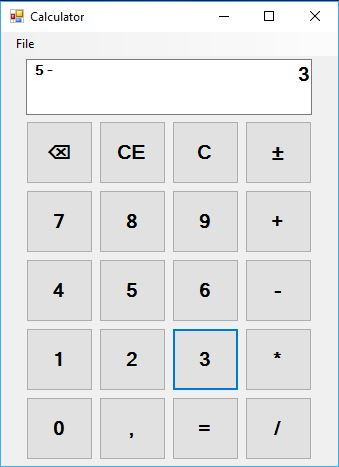
\includegraphics{Cattura.JPG}

\clearpage

2. Calculator stiintifc

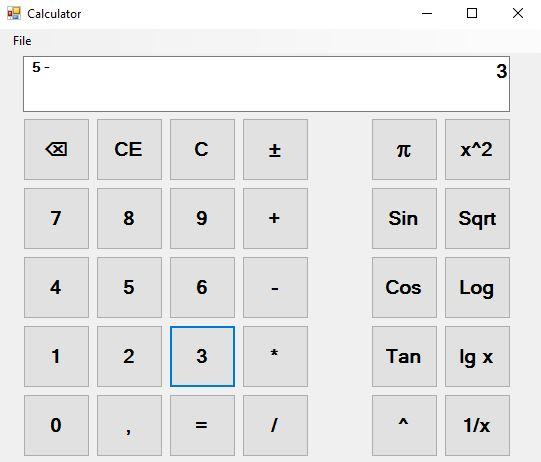
\includegraphics{Cattura1.JPG}

\clearpage

3. Istoria


\includegraphics{Cattura2.JPG}




\clearpage
        
